\begin{frame}
\begin{example} 
Where is this function discontinuous?
\begin{columns}[c]
\column{.4\textwidth}
\[
f(x) = \left\{ \begin{array}{lcl}
\frac{1}{\alertNoH{6}{x^2}} & \text{ if } & x \neq 0 \\
\alertNoH{4}{1} & \alertNoH{4}{\text{ if }} & \alertNoH{4}{x = 0} \\
\end{array}\right.
\]
\psset{xunit=0.7cm, yunit=0.7cm}
\begin{pspicture}(-3.2, -0.5)(3.2,7.1) 
\psframe*[linecolor=white](-3.1,-0.5)(3.1,7.1)
\psaxes[ticks=x, labels=none]{<->}(0,0)(-3,-0.5) (3,7)
\psplot[linecolor=red, plotpoints=1000]{1 7.09 div sqrt}{3}{1 x 2 exp div }
\psplot[linecolor=red, plotpoints=1000]{-3}{1 7.09 div sqrt -1 mul}{1 x 2 exp div}
\rput(2,2){$y=\frac{1}{x^2}$}
\fcFullDot{0}{1}
\end{pspicture} %
%\ 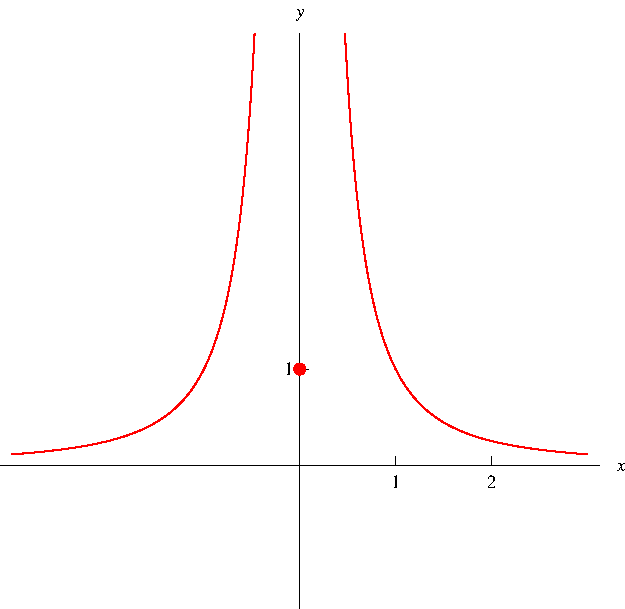
\includegraphics[height=4.5cm]{continuity/pictures/02-05-ex2b.pdf}%
\column{.6\textwidth}
\begin{itemize}
\item<2-| alert@3-4>  $f(0)$ \fcAnswer{4}{is defined ($f(0) = 1$).}
\item<2-| alert@5-6>  $\lim\limits_{x\rightarrow 0} f(x)$ \fcAnswer{6}{doesn't exist ($\infty$).}
\item<7->  Discontinuous at 0.
\item<8->  This is called an infinite discontinuity.
\end{itemize}
\end{columns}
\end{example}
\end{frame}